\begin{figure}
\begin{center}
    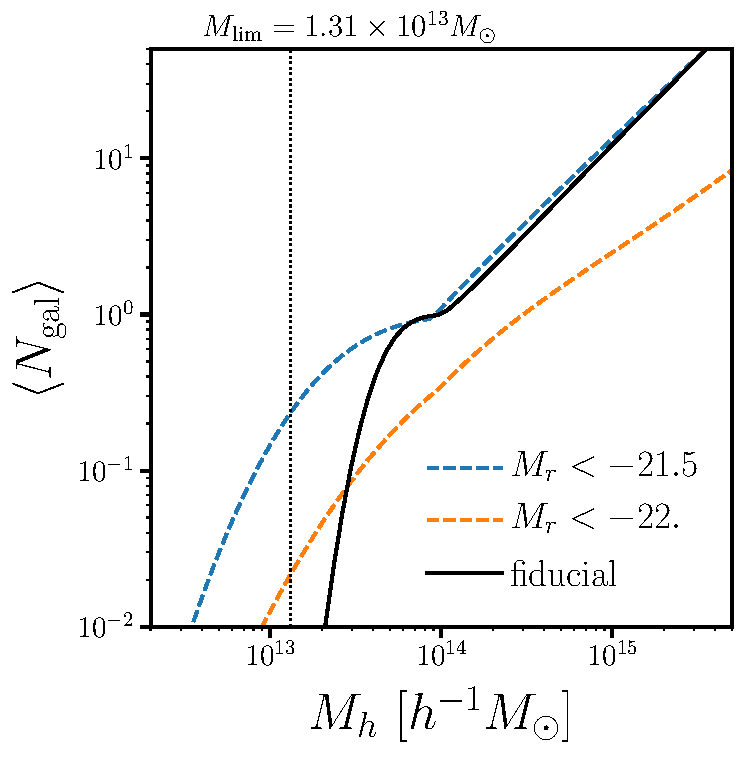
\includegraphics[width=0.75\textwidth]{figs/hod_fid.pdf} 
    \caption{

    }\label{fig:hod}
\end{center}
\end{figure}

\section{Halo Occupation Distribution} \label{sec:hod}  
We're interested in quantifying the information content of the galaxy 
bispectrum. With a perturbation theory approach, this would involve 
incorporating a bias model for galaxies~\citep[\emph{e.g.}][]{sefusatti2006, yankelevich2019, chudaykin2019}. 
Instead, for our simulation driven approach, we use the halo occupation 
distribution (HOD) framework~\citep[\emph{e.g.}][]{zheng2005,leauthaud2012,tinker2013,zentner2016,vakili2019}. 
The HOD model specifies how 

\bitem
\item description of HODs in general and how we're going to use them our bias model. 
    This is the framework used to construct simulated mock catalogs and used 
    ubiquitously in galaxy clustering analyses. Moreover, it's used for emulator 
    set ups (Aemulus), which as we mention earlier is the only hopes for accurately 
    modeling the high k.
\item We use the standard \cite{zheng2007} model, which has been used extensively. 
    Discuss the obvious shortcomings of the model. However, \cite{vakili2019} did not 
    find strong evidence for assembly bias and we're going for simplicity here. 
\item description of the halo mass constraints we're dealing with and how this prevents 
    us from directly using best-fit HOD parameters from the literature. In fact, due
    to this constraint we modify the HOD parameters.
\item plots showing how our HOD choice compares to HODs of the SDSS samples. Some handwavy
    arguments about how it shouldn't matter too much. 
\eitem

% --- excerpt from Hahn et al. (2017) --- 
%The foundation of HOD predictions is the halo model of LSS, that is, collapsed dark matter halos are biased tracers of the underlying cos- mic density field (Press & Schechter 1974; Bond et al. 1991; Cooray & Sheth 2002). The HOD specifies how the dark matter halos are populated with galaxies by modeling the probability that a given halo hosts N galaxies subject to some observational selection criteria (Lemson & Kauffmann 1999; Seljak 2000; Scoccimarro et al. 2001; Berlind & Wein- berg 2002; Zheng et al. 2005). This statistical prescription for connecting galaxies to halos has been remarkably successful in reproducing the galaxy clustering, galaxy–galaxy lensing, and other observational statistics (Rodr ́ıguez-Torres et al. 2015; Miyatake et al. 2015), and is a useful framework for constraining cosmological parameters (van den Bosch et al. 2003; Tinker et al. 2005; Cacciato et al. 2013; More et al. 2013) as well as galaxy evolution models (Conroy & Wech- sler 2009; Tinker et al. 2011; Leauthaud et al. 2012; Behroozi et al. 2013b; Tinker et al. 2013, Walsh et al. in preparation).

% --- excerpt from Zhai et al. (2018) --- 
%Retrieving information from these scales has been a goal of modern cosmology, but it has also been a challenge. Non- linear dynamics of dark matter are captured with excellent precision in modern cosmological N-body simulations (see, e.g., Klypin et al. 2011, 2016). The challenge of constraining cosmology with such simulations is two-fold: (1) an accu- rate and flexible model of the galaxy bias is required, and (2) one needs to be able to properly sample cosmological pa- rameter space, which becomes computationally intractable for a standard Monte Carlo Markov Chain analysis. Be- cause of these limitations, the amount of information that is extractable from small-scale galaxy clustering is simply unknown. The measurement precision of the data is orders of magnitude higher than at large scales, but the theoretical complexity increases significantly. How much information is recoverable after accounting for all possibilities in galaxy bias? In this paper, for the case of RSD, we will show that af- ter marginalizing over numerous galaxy bias parameters and incorporating the theoretical uncertainty in the galaxy clus- tering model, it is still possible to extract more constraining power from growth of structure measurements than what is achievable using perturbation theory on large scales.
%To solve problem (1), we use the halo occupation distri- bution (HOD; Berlind & Weinberg 2002; Peacock & Smith 2000; Seljak 2000; Benson et al. 2000; White et al. 2001; Cooray & Sheth 2002). The HOD approaches galaxy bias by quantifying the statistical relationship between galaxies and dark matter halos. In its most basic form, the HOD is mostly determined by the probability distribution P(N|M), the prob- ability that a halo of mass M contains N galaxies of a given class. Once P(N|M) is combined with prescriptions for spa- tial and velocity bias of galaxies within halos, this model of- fers nearly a complete description of the spatial distribution of galaxies for a given halo population. This simple approach of P(N|M), however, ignores the possibility that N may de- pend on some secondary halo property. If this halo property is correlated with the spatial distribution of halos, this could create a ‘galaxy secondary bias’ (also known as galaxy as- sembly bias) that would have to be incorporated in the prob- ability distribution in order to create a fully descriptive HOD (Sheth & Tormen 2004; Gao et al. 2005; Harker et al. 2006; Wechsler et al. 2006). The optimal method for incorporating galaxy assembly bias into the HOD, and tests against models that contain these effects, is left to another paper (McLaugh- lin et al. 2018). Our emphasis here is on determining the to- tal constraining power and the scales from which these con- straints come, under the assumption that the assumed HOD approach is sufficient for modeling galaxy bias.
